\chapter{Analysis of performance}

\pgfplotsset{
	every axis/.append style={
		line width=.5 pt,
		tick style={line width=.6pt},
		label style={font=\footnotesize},
		tick label style={font=\footnotesize},
	}
}

The time of the simulation will be used to characterize the performance when 
several parameters are changed. The time is measured using the wall clock, and 
refers to the \textit{time per iteration}. Sometimes the different stages of the 
simulator will be measured as well, to give more insight in the distribution of 
the time. Notice that each process may start or end a iteration at different 
times, by in the long run all processes must be synchronized. The measurements 
will take place only in the first process (with rank zero).

At each iteration various factors may affect the iteration time and introduce a 
random delay. We will model the simulation time as $t = \hat t + e_t$, where the 
true simulation time $\hat t$ is unknown but constant between iterations, and 
the error $e_t$ is a random variable with zero mean and unknown but finite 
variance $\sigma^2$.  Additionally, we will assume that the error $e_t$ is 
independent and identically distributed in each iteration of the same 
configuration and that follows a normal distribution.

We can then consider the sequence of measured times $T = t_1,\ldots,t_n$ as 
independent random variables from a common distribution with an unknown mean 
$\hat t$ and finite standard deviation $\sigma$. The sample mean $\overline T$ 
can be approximated with a certain degree of confidence by a process of 
sampling. The standard error of the mean (SEM) will be used to get a confidence 
interval in which we can ensure the true mean is located. The standard error of 
the mean (SEM) is defined as
%
\begin{equation}
\epsilon = \frac{\sigma}{\sqrt{n}}
\end{equation}
%
As the standard deviation $\sigma$ is unknown, following the assumption that the 
error follows a normal distribution, we can use the student distribution to get 
the standard error using the standard deviation of the sample $s$
%
\begin{equation}
\epsilon = Z_\alpha\frac{s}{\sqrt{n}}
\end{equation}
%
With a significance level $\alpha=0.05$ we get from the t-student distribution 
the value $Z=1.96$, and we can obtain the confidence interval $\overline T \pm 
\epsilon$ where we can ensure the true mean is located with a probability of 
95\%. By setting the relative error $\delta = \epsilon / \overline T$ to be 
lower than 1\%, we obtain the limit error $\epsilon_0$ to be $\epsilon_0 = 0.01 
\overline T$.
%
Then, if we stop the simulation process when the standard error of the mean is 
below $\epsilon_0$
%
\begin{equation}
\epsilon = Z_\alpha\frac{s}{\sqrt{n}} < 0.01 \, \overline T
\end{equation}
%
We can ensure that (a) with probability 0.95 the true mean $\hat t$ is located 
in the interval $\overline T \pm \epsilon$, and (b) the relative error of the 
mean $\delta$ is lower than 1\%.

The process of simulation will run for at least a minimum of 30 iterations. Then 
it will continue until the relative error is below 1\%, or the simulation time 
exceeds 30 minutes.
%
All experiments were run in Mare Nostrum 4, using Intel MPI and the Intel 
\texttt{icc} compiler with the following modules:
%\setlength{\columnsep}{-2.1in}
\begin{multicols}{3}
\begin{itemize}
\item intel/2017.4
\item fftw/3.3.6
\item tampi/1.0
\item impi/2017.4
\item ompss-2/2019.06
\item extrae/3.7.0
\end{itemize}
\end{multicols}

%
\vspace{1em}
\todo[inline]{Use error bars to denote CI at 95\% not std?}

\section{Performance model}

Consider the real time of the simulation $\hat t(c)$ to be a function of a 
specific configuration $c$. There are a lot of parameters that may be changed 
and have some influence in the time per iteration, but we will focus only on the 
following ones.
%
\begin{itemize}
\item $N_p$: Number of total particles.
\item $N_g$: Number of total grid points.
\item $N_c$: Number of plasma chunks.
\item $P$: Number of total MPI processes.
\item $C$: Number of total cores.
\item $A$: Whether TAMPI ($A = 1$) or MPI ($A=0$) is being used.
\end{itemize}
%
A configuration is then completely specified as the tuple $c = (N_p, N_g, N_c, 
P, C, A)$. The space of states of configurations possible is bigger than the 
available time for experimentation, so we must choose a partial group which can 
reveal interesting information of the effect in the iteration time.
%
\subsection{Number of particles}

The number of particles $N_p$ is one of the main parameters that affect the
running time of each iteration as it can be observed from the simulation process 
that at least a complexity in $O(N_p)$ is expected---we need to cycle through 
each particle at every iteration. To get an accurate relation, an experiment is 
run sweeping from \num{2e6} to \num{4e7} particles, with 32 cores and only one 
process. The number of grid points is kept low at $1024^2$ in order to avoid 
interference from the solver. We see in the figure~\ref{fig:particles-32cpus} 
how the time scales linearly with the number of particles, and the residuals of 
the linear regression. With a determination coefficient of $R^2 = 0.99981$, we 
can estimate a time per particle of \SI{51.4}{\micro\second} with 32 cores.

\begin{figure}[h]%{{{
	\centering
	\begin{tikzpicture}
	\begin{axis}[
		width=0.5\textwidth,
		xlabel=Particles $N_p$,
		ylabel=Time per iteration (s),
		no markers,
		%grid=major,
	]
	\addplot [only marks,scatter,error bars/y dir=both, error bars/y explicit] 
	table [
		x index = {0},
		y index = {3},
		y error index={4},
		col sep=space] {perf/particles/csv/time.csv};
	\addplot [red] table [col sep=space] {perf/particles/csv/regression.csv};
	\end{axis}
	\end{tikzpicture}
	\begin{tikzpicture}
	\begin{axis} [
		yticklabel pos=right,
		xlabel=Particles $N_p$,
		ylabel=Residuals (s),
		width=0.5\textwidth,
		%grid=major,
	]
	\addplot [
		only marks,
		error bars/y dir=both,
		error bars/y explicit,
	] table [
		x index = {0},
		y index = {2},
		y error index = {3},
		col sep=space] {perf/particles/csv/regression.csv};
	\draw[
		ultra thin,
		black!30!white
	] (axis cs:\pgfkeysvalueof{/pgfplots/xmin},0) --
			(axis cs:\pgfkeysvalueof{/pgfplots/xmax},0);
	\end{axis}
	\end{tikzpicture}
	\caption{The number of particles $N_p$ is increased and the time per iteration 
	$t$ is measured. A linear regression fit is shown, with the residuals at the 
	left. Using one process and 32 CPUs MPI communications are not needed.  
	Configuration used ($N_p=\num{2e6}\text{ to }\num{4e7}$, $N_g = 1024^2$, 
	$N_c=128$, $P=1$, $C=32$, $A=1$)}
	\label{fig:particles-32cpus}
\end{figure}%}}}

\subsection{Number of grid points}

The MFT solver uses the FFTW library to perform the FFT and solve the field 
equation in each iteration, with an expected worst time complexity in $O(N_g 
\log N_g)$. An experiment with varying number of grid points from $2048^2$ to 
$8192^2$ is designed to observe the grow in time.
%
\begin{figure}[h]%{{{
	\centering
	\begin{tikzpicture}
	\begin{axis} [
			no markers,
			grid=major,
			xlabel=Grid points $N_g$,
			ylabel=Time per iteration (s),
			width=0.5\textwidth]
		\addplot [scatter,only marks,error bars/y dir=both, error bars/y explicit] 
		table [
			x index = {0},
			y index = {3},
			y error index={4},
			col sep=space] {perf/gridpoints/time.csv};
		\addplot [red] table [col sep=space] {perf/gridpoints/csv/regression.csv};
	\end{axis}
	\end{tikzpicture}
	\begin{tikzpicture}
	\begin{axis} [
		yticklabel pos=right,
		xlabel=Particles $N_p$,
		ylabel=Residuals (s),
		width=0.5\textwidth,
		%grid=major,
	]
	\addplot [
		only marks,
		error bars/y dir=both,
		error bars/y explicit,
	] table [
		x index = {0},
		y index = {2},
		y error index = {3},
		col sep=space] {perf/gridpoints/csv/regression.csv};
	\draw[
		ultra thin,
		black!30!white
	] (axis cs:\pgfkeysvalueof{/pgfplots/xmin},0) --
			(axis cs:\pgfkeysvalueof{/pgfplots/xmax},0);
	\end{axis}
	\end{tikzpicture}
	\caption{The effect of the variables $N_p$ and $N_g$ to the time per 
	iteration. Using one process and 32 CPUs (MPI communications are not needed).}
	\label{fig:gridpoints-32cpus}
\end{figure}%}}}
%
In the figure~\ref{fig:gridpoints-32cpus} it can be seen how the time grows with 
the number of grid points, but the variance is much bigger than with the number 
of particles. Notice that the dispersion is not due to random variations in the 
execution time, as the standard deviation for each point is lower than its 
dispersion from the common distribution. The FFTW uses an algorithm which 
benefits from sizes that can be decomposed into the product of small multiples 
($2^a \cdot 3^b\cdot 5^c\cdot 7^d\,\ldots$).  However the number of points in 
the X axis must be divisible by the number of plasma chunks, and some of the 
sizes tested had large primes in their decomposition.
%
\todo[inline]{Regenerate figure with appropriate sizes and check the dispersion 
decreases.}
%

\section{Solver multithreading scalability}

The simulator is designed to scale with the number of particles when the number 
of cores or MPI processes are incremented---each chunk can be computed in 
parallel both in the X and Y axis. But when the number of grid points is 
incremented, the FFT solver must scale both in the number of CPUs and processes.  

The space in Y is divided into equally sized blocks, which are assigned into MPI 
processes, following the parallelization design of the FFTW. Additionally the 
library offers two parallelization implementations for multithreading: Using 
OpenMP and POSIX threads (pthreads).  OpenMP is not compatible with OmpSs-2 as 
we have one runtime already running so the pthread implementation was tested.
%
\begin{figure}[h]%{{{
	\centering
		\begin{tikzpicture}
		\begin{axis} [
			legend pos=north west,
			xmode=log,
			log basis x=2,
			xticklabels={0,1,2,4,8,16,32},
			grid=major,
			xlabel=Number of CPUs,
			ylabel=Time per iteration (s),
			width=10cm,
			height=6cm,
			]
		\addplot+ [error bars/y dir=both, error bars/y explicit] table [
			x index = {0},
			y index = {3},
			y error index={4},
			col sep=space] {perf/fftw-sequential/time.csv};
		\addlegendentry{Single thread}
		\addplot+ [error bars/y dir=both, error bars/y explicit] table [
			x index = {0},
			y index = {3},
			y error index={4},
			col sep=space] {perf/fftw-threads/time.csv};
		\addlegendentry{Multithread}
		\end{axis}
		\end{tikzpicture}
	\caption{The number of CPUs is increased with only one process: the solver 
	cannot scale and the time per iteration increases. Configuration used: $N_p = 
	\num{5e5}$, $N_g=8192\times8192$.}
	\label{fig:fftw-time}
\end{figure}%}}}
%
Unfortunately, the FFTW library doesn't show a good speedup, in fact worsens the 
time per iteration when adding more threads with the configurations tested. In 
the figure~\ref{fig:fftw-time} it can be shown how the time grows as the number 
of CPUs increases.
%
The FFTW documentation warns about this problem, claiming that it can only 
improve the time with large enough matrices:
%
\begin{displayquote}
A shared-memory machine is one in which all CPUs can directly access the same 
main memory, and such machines are now common due to the ubiquity of multi-core 
CPUs. FFTW’s multi-threading support allows you to utilize these additional CPUs 
transparently from a single program. However, this does not necessarily 
translate into performance gains---when multiple threads/CPUs are employed, 
there is an overhead required for synchronization that may outweigh the 
computational parallelism. Therefore, you can only benefit from threads if your 
problem is sufficiently large.
\end{displayquote}
%
However, larger matrices are not useful to get more precise results, as we 
rather prefer an increase the number of particles than grid points.


\begin{figure}[h]%{{{
	\centering
	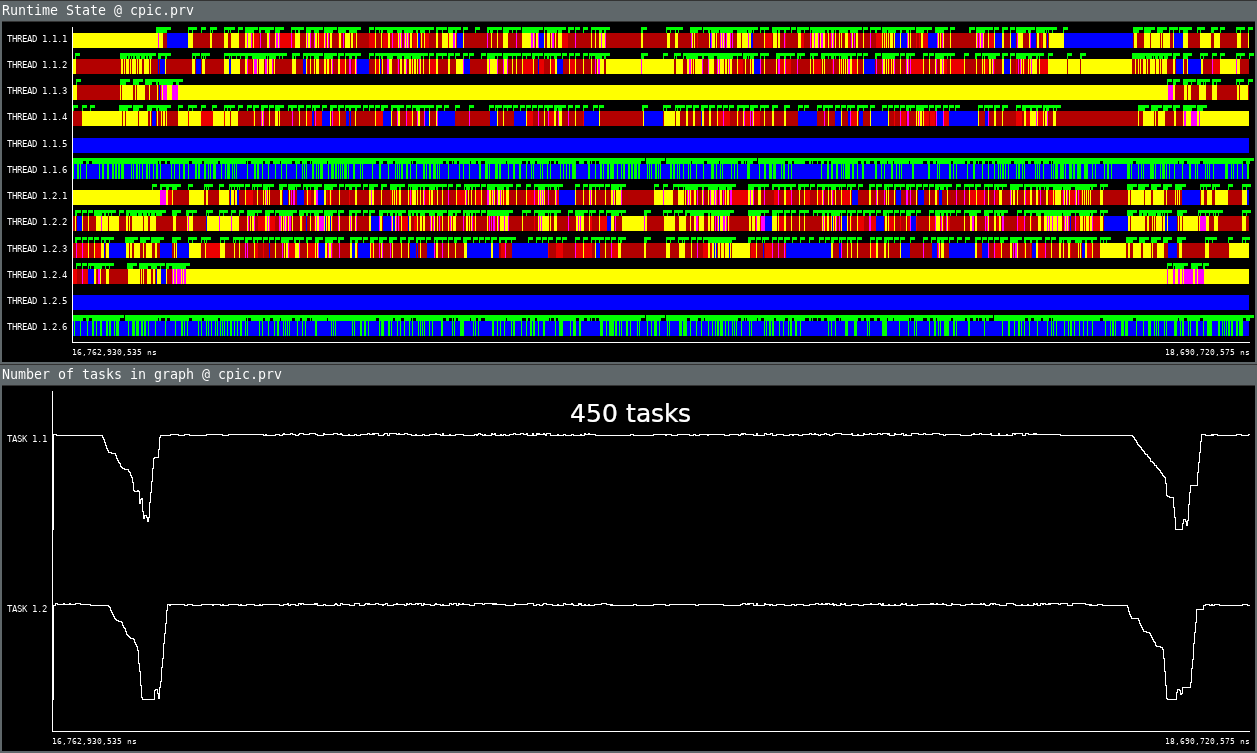
\includegraphics[width=0.95\linewidth]{fftw-ompss2.png}
	\caption{Tasks created inside the FFTW when using OmpSs-2: Up to 450 tasks are 
	created in rapid succession, with only 4 CPUs and 2 processes.}
	\label{fig:fftw-ompss2}
\end{figure}%}}}

In order to avoid a scalability problem, another approach was tested: Add 
support for OmpSs-2~in the FFTW to enable multithreading, following the same 
structure as OpenMP. The results obtained were similar as with the pthread case, 
but more insight was gained in how the task were being created. It shown that 
the overhead added by the large amount of created and destructed quick tasks 
outweight any benefit that could be gained by multithreading.

We can mitigate the effect of the scaling by increasing the number of processes.  
In order to evaluate which ratio of processes and CPUs yields the best 
performance several configurations are tested. With a fixed number of maximum 
CPUs available set to 32, we increase the number of processes while we reduce 
the CPUs per process.

\begin{figure}[h]%{{{
	\centering
		\begin{tikzpicture}
		\begin{axis} [
			legend pos=outer north east,
			xmode=log,
			log basis x=2,
			xticklabels={0,1,2,4,8,16},
%			xticklabel style={
%			/pgf/number format/precision=3,
%			/pgf/number format/fixed},
			grid=major,
			xlabel=Number of CPUs per process,
			ylabel=Time per iteration (s),
			width=0.5\textwidth]
		\addplot [ybar stacked, fill=red!30!white] table [
			x index = {0},
			y index = {10},
			col sep=space] {perf/constant-cpus/time.csv};
		\addlegendentry{Solver}
		\addplot [ybar stacked, fill=blue!30!white] table [
			x index = {0},
			y index = {11},
			col sep=space] {perf/constant-cpus/time.csv};
		\addlegendentry{Particles}
		\addplot [only marks,error bars/y dir=both, error bars/y explicit] table [
			x index = {0},
			y index = {5},
			y error index={6},
			col sep=space] {perf/constant-cpus/time.csv};
		\addlegendentry{Total}
		\end{axis}
		\end{tikzpicture}
	\caption{The number of CPUs per process is incremented while reducing the 
	number of processes (the total number of CPUs is set to 32 and is kept 
	constant).  The time per iteration is measured, which leads to a 
	characteristic U shape.}
	\label{fig:fftw-u}
\end{figure}%}}}

%\begin{figure}[h]{{{
%	\centering
%		\begin{tikzpicture}
%		\begin{axis} [
%			baseline,
%			xmode=log,
%			log basis x=2,
%			xticklabels={0,1,2,4,8,16},
%%			xticklabel style={
%%			/pgf/number format/precision=3,
%%			/pgf/number format/fixed},
%			grid=major,
%			xlabel=Number of CPUs per process,
%			ylabel=Time per iteration (s),
%			ymax=6,
%			width=0.5\textwidth,
%			height=10cm,
%			]
%		\foreach \Nc in {32,64,128,256,512} {
%			\edef\temp{\noexpand\addlegendentry{$N_c = \Nc$}}
%			\addplot+ table [
%				x = P,
%				y = mean,
%				y error = {rel-err},
%				col sep=tab] {csv/mpi-scaling/Nc\Nc};
%			%\temp
%		}
%		\end{axis}
%		\end{tikzpicture}
%		\hspace{0.15cm}
%		\begin{tikzpicture}
%		\begin{axis} [
%			baseline,
%			xmode=log,
%			log basis x=2,
%			xticklabels={0,1,2,4,8,16},
%%			xticklabel style={
%%			/pgf/number format/precision=3,
%%			/pgf/number format/fixed},
%			grid=major,
%			xlabel=Number of CPUs per process,
%			ylabel=Time per iteration (s),
%			height=10cm,
%			width=0.5\textwidth]
%		\foreach \Nc in {32,64,128,256,512} {
%			\edef\temp{\noexpand\addlegendentry{$N_c = \Nc$}}
%			\addplot+ table [
%				x = P,
%				y = mean,
%				y error = {rel-err},
%				col sep=tab] {csv/tampi-scaling/Nc\Nc};
%			\temp
%		}
%		\end{axis}
%		\end{tikzpicture}
%	\caption{The number of CPUs per process is incremented while reducing the 
%	number of processes (the total number of CPUs is set to 32 and is kept 
%	constant).  The time per iteration is measured, which leads to a 
%	characteristic U shape.}
%\end{figure}}}}

\section{TAMPI}

The two modes of communication are compared with different configurations, in 
order to evaluate the effect in the overall performance of the simulation. The 
chunk size $N_c$ determines the number of messages sent per process and is 
tested from 32 to 512.
%
\begin{figure}%{{{
\centering
\begin{tikzpicture}
	\begin{groupplot}[
		group style={
			columns=2,
%			rows=2,
			horizontal sep=0.5cm,
			ylabels at=edge left,
			yticklabels at=edge left,
		},
		xmode=log,
		log basis x=2,
%		xticklabels={0,1,2,4,8,16},
		grid=major,
		xmin=0,
		ymin=0,
		xlabel=Number of processes,
		ylabel=Time per iteration (s),
		height=10cm,
		width=7cm,
		/tikz/font=\small]
	\nextgroupplot[
		ymax=6,
		title={MPI},
%		error bars/y dir=both,
%		error bars/y explicit
	]
	\foreach \Nc in {32,64,128,256,512} {
		\edef\temp{\noexpand\addlegendentry{$N_c = \Nc$}}
		\addplot+ table [
			x = P,
			y = mean,
			y error = {rel-err},
			col sep=tab] {perf/mpi-scaling/csv/Nc\Nc};
		%\temp
	}
% Using inout is slightly slower than commutative
%	\nextgroupplot[ymax=6,title={MPI with inout}]
%	\foreach \Nc in {32,64,128,256,512} {
%		\edef\temp{\noexpand\addlegendentry{$N_c = \Nc$}}
%		\addplot+ table [
%			x = P,
%			y = mean,
%			y error = {rel-err},
%			col sep=tab] {csv/mpi-inout-scaling/Nc\Nc};
%		%\temp
%	}
	\nextgroupplot[
		ymax=6,
		title={TAMPI},
%		error bars/y dir=both,
%		error bars/y explicit
	]
	\foreach \Nc in {32,64,128,256,512} {
		\edef\temp{\noexpand\addlegendentry{$N_c = \Nc$}}
		\addplot+ table [
			x = P,
			y = mean,
			y error = {rel-err},
			col sep=tab] {perf/tampi-scaling/csv/Nc\Nc};
		\temp
	}
	\end{groupplot}
\end{tikzpicture}
\caption{Comparison of MPI and TAMPI}
\label{fig:TAMPI}
\end{figure}%}}}
%
In the figure~\ref{fig:TAMPI} it can be seen how the time is drastically reduced 
when TAMPI is enabled. The performance difference is lower when the number of 
processes increases, but is very significant with few processes. Notice the 
control case with only one process were no MPI nor TAMPI communication is needed 
(shared memory is used to exchange information between tasks).

It is also noted with MPI a saturation point with 512 chunks per process, where 
the time does not improve with more processes. Different versions of OpenMPI 
(3.1.1, 4.0.0 and 4.0.1) were also tested, and there was a extreme delay of more 
than one order of magnitude with respect to the mean time per iteration with low 
probability of occurrence, and the causes are yet unknown. The same problem was 
never observed with Intel MPI, but further investigation is needed to isolate 
the issue and conclude that is due to OpenMPI.

\section{Scalability}

In order to evaluate the simulator in terms of scalability the two main metrics 
are initially measured:
\begin{enumerate}
\item \textbf{Strong scalability}: The same configuration of problem is repeated 
with increasing number of computing elements.
\item \textbf{Weak scalability}: The number of computing elements is increased, 
while the amount of work assigned to each one is kept constant by changing the 
problem configuration.
\end{enumerate}
%
%
\begin{figure}[ht]%{{{
\centering
\begin{tikzpicture}
	\begin{axis}[
		xmode=log,
		log basis x=2,
		xticklabels={0,1,2,4,8,16,32},
		grid=major,
		xmin=0,
		ymin=0,
		xlabel=Number of nodes,
		ylabel=Speedup,
		height=8cm,
		width=0.5\textwidth,
		/tikz/font=\small]
		\addplot+ table [
			x = P,
			y = speedup,
			col sep=tab] {perf/strong-scaling-fixed/csv/time.csv};
	\end{axis}
\end{tikzpicture}
\begin{tikzpicture}
	\begin{axis}[
		xmode=log,
		log basis x=2,
		xticklabels={0,1,2,4,8,16,32},
		grid=major,
		xmin=0,
		ymin=0,
		xlabel=Number of nodes,
		ylabel=Efficiency,
		height=8cm,
		width=0.5\textwidth,
		/tikz/font=\small]
		\addplot+ table [
			x = P,
			y = efficiency,
			col sep=tab] {perf/strong-scaling-fixed/csv/time.csv};
	\end{axis}
\end{tikzpicture}
	\caption{Strong scaling with configuration: $N_p = \num{1e8}$, $N_g = 2048^2$,
	$N_c = 128$, one process per node, using each 48 cores.}
	\label{fig:strong-scaling}
\end{figure}%}}}
%
For the strong scalability, a fixed configuration of $N_p = \num{1e8}$ 
particles, $N_g=2048^2$ grid points and $N_c=128$ chunks is used to run the 
simulator with increasing number of computing nodes. Each node runs with 48 
cores---all the available CPUs of the machine. In the 
figure~\ref{fig:strong-scaling} the speedup and the efficiency are shown.
The rapid decay of efficiency is to be expected, as the solver cannot exploit 
the full 48 cores and only one is used when solving the FFT. We can obtain more 
information of the scalability of the simulator without the solver by disabling 
it---the physical result of the simulation will be non-sense, but the same 
stages of the simulator will be executed as if the solver was enabled. We see in 
the figure~\ref{fig:strong-scaling-without-solver} how the efficiency now 
improves substantially, and indicates that the solver is acting as a bottle neck 
which leads to a significant reduction in scalability.
%
\begin{figure}[ht]%{{{
\centering
\begin{tikzpicture}
	\begin{axis}[
		xmode=log,
		log basis x=2,
		xticklabels={0,1,2,4,8,16,32},
		grid=major,
		xmin=0,
		ymin=0,
		xlabel=Number of nodes,
		ylabel=Speedup,
		height=8cm,
		width=0.5\textwidth,
		/tikz/font=\small]
		\addplot+ table [
			x = P,
			y = speedup,
			col sep=tab] {perf/strong-scaling-fixed-without-fft/csv/time.csv};
	\end{axis}
\end{tikzpicture}
\begin{tikzpicture}
	\begin{axis}[
		xmode=log,
		log basis x=2,
		xticklabels={0,1,2,4,8,16,32},
		grid=major,
		xmin=0,
		ymin=0,
		xlabel=Number of nodes,
		ylabel=Efficiency,
		height=8cm,
		width=0.5\textwidth,
		/tikz/font=\small]
		\addplot+ table [
			x = P,
			y = efficiency,
			col sep=tab] {perf/strong-scaling-fixed-without-fft/csv/time.csv};
	\end{axis}
\end{tikzpicture}
	\caption{Strong scaling with the solver disabled (the physical simulation is 
	incorrect without the solver, but the other stages of the simulation are 
	properly executed as if they were genuine).  Using the same configuration: 
	$N_p = \num{1e8}$, $N_g = 2048^2$,
	$N_c = 128$, one process per node, using each 48 cores.}
	\label{fig:strong-scaling-without-solver}
\end{figure}%}}}
%

In order to analyze the weak scalability, a configuration is prepared to remain 
with constant work per computing elements (we will use the number of nodes, as 
each one will run at full capacity, using the 48 CPUs). The configuration chosen 
has \num{1e7} particles per CPU or \num{4.8e8} per node. The number of chunks is 
set to 128 and the number of grid points to $2048^2$. Similarly as for the 
strong scalability, the number of nodes is tested from 1 to 32, in powers of 2.
%
\begin{figure}%{{{
\centering
\begin{tikzpicture}
	\begin{axis}[
		xmode=log,
		log basis x=2,
		xticklabels={0,1,2,4,8,16,32},
		grid=major,
		xmin=0,
		ymin=0,
		xlabel=Number of nodes,
		ylabel=Efficiency,
		%height=10cm,
		%width=0.5\textwidth,
		/tikz/font=\small]
		\addplot+ table [
			x = P,
			y = speedup, %TODO: Fix the column name
			col sep=tab] {perf/weak-scaling/csv/time.csv};
	\end{axis}
\end{tikzpicture}
\caption{Weak scaling with \num{1e7} particles per CPU.}
\label{fig:weak-scaling}
\end{figure}%}}}
%
In the figure~\ref{fig:weak-scaling} the simulator shows a steady efficiency, 
which slowly decreases after the 8 nodes.

\todo[inline]{Test weak scaling with constant $N_g$ per CPU.}

\section{Extended scalability}

In order to get more information when other parameters vary, more experiments 
were designed to show the effect in the efficiency. The solver is one of the 
main factors that adversely affect the iteration time, which can be mitigated by 
varying the ratio of CPUs per process, with the drawback of increasing the 
overhead in the other phases of the computation that benefit from shared memory 
communication, as identified in the figure~\ref{fig:fftw-u}.

\todo[inline]{Complete this}

%\begin{figure}%{{{
%\centering
%\begin{tikzpicture}
%	\begin{groupplot}[
%		group style={
%			columns=3,
%			rows=2,
%			horizontal sep=0.5cm,
%			ylabels at=edge left,
%			yticklabels at=edge left,
%		},
%		legend pos=outer north east,
%		xmode=log,
%		log basis x=2,
%%		xticklabels={0,1,2,4,8,16},
%		grid=major,
%		ymin=0,
%		xlabel=Number of processes,
%		ylabel=Efficiency,
%		height=10cm,
%		width=5cm,
%		/tikz/font=\small]
%	\nextgroupplot[title={32 chunks}]
%	\foreach \CP in {1,2,4,8,16,32,48} {
%		\edef\temp{\noexpand\addlegendentry{\CP}}
%		\addplot+ table [
%			x = P,
%			y = efficiency,
%			y error = {rel-err},
%			col sep=tab] {perf/strong-scaling/csv/CP\CP-Nc32};
%%		\temp
%	}
%	\nextgroupplot[title={64 chunks}]
%	\foreach \CP in {1,2,4,8,16,32,48} {
%		\edef\temp{\noexpand\addlegendentry{\CP}}
%		\addplot+ table [
%			x = P,
%			y = efficiency,
%			y error = {rel-err},
%			col sep=tab] {perf/strong-scaling/csv/CP\CP-Nc64};
%%		\temp
%	}
%	\nextgroupplot[title={128 chunks}]
%	\addlegendimage{empty legend}
%	\addlegendentry{\hspace{-0.6cm}$CPUs/P$}
%	\foreach \CP in {1,2,4,8,16,32,48} {
%		\edef\temp{\noexpand\addlegendentry{\CP}}
%		\addplot+ table [
%			x = P,
%			y = efficiency,
%			y error = {rel-err},
%			col sep=tab] {perf/strong-scaling/csv/CP\CP-Nc128};
%		\temp
%	}
%	\end{groupplot}
%\end{tikzpicture}
%\end{figure}%}}}



\begin{figure}%{{{
\centering
\begin{tikzpicture}
	\begin{groupplot}[
		group style={
			columns=3,
			rows=2,
			horizontal sep=0.5cm,
			ylabels at=edge left,
			yticklabels at=edge left,
		},
		legend pos=outer north east,
		xmode=log,
		log basis x=2,
%		xticklabels={0,1,2,4,8,16},
		grid=major,
		ymin=0,
		ymax=1.25,
		xlabel=Number of CPUs,
		ylabel=Efficiency,
		height=10cm,
		width=5cm,
		/tikz/font=\small]
	\nextgroupplot[title={1 CPU/process}]
	\foreach \ng in {1024,2048,4096,8192,16384} {
		\edef\temp{\noexpand\addlegendentry{\ng}}
		\addplot+ table [
			x = C,
			y = efficiency,
			y error = {rel-err},
			col sep=tab] {perf/gridpoints-scaling/csv/CP1-ng\ng};
%		\temp

	}
	\nextgroupplot[title={16 CPUs/process}]
	\foreach \ng in {1024,2048,4096,8192,16384} {
		\edef\temp{\noexpand\addlegendentry{\ng}}
		\addplot+ table [
			x = C,
			y = efficiency,
			y error = {rel-err},
			col sep=tab] {perf/gridpoints-scaling/csv/CP16-ng\ng};
%		\temp
	}
	\nextgroupplot[title={32 CPUs/process}]
	\addlegendimage{empty legend}
	\addlegendentry{\hspace{-0.6cm}$N_g$}
	\foreach \ng in {1024,2048,4096,8192,16384} {
		\edef\temp{\noexpand\addlegendentry{$\ng^2$}}
		\addplot+ table [
			x = C,
			y = efficiency,
			y error = {rel-err},
			col sep=tab] {perf/gridpoints-scaling/csv/CP32-ng\ng};
		\temp
	}
	\end{groupplot}
\end{tikzpicture}

\end{figure}%}}}
